\begin{frame}
  \frametitle{API REST}

  \begin{itemize}
  \item Ideazione da parte di Roy Fielding negli anni 2000
  \item Linee guida:
    \begin{itemize}
    \item Identificazione delle risorse
    \item Utilizzo esplicito dei metodi HTTP
    \item Risorse autodescrittive
    \item Collegamenti tra risorse
    \item Comunicazioni prive di stato
    \end{itemize}
  \end{itemize}

  \begin{figure}[H]
    \centering
    
\includegraphics[scale=0.2]{rest-api}
  \end{figure}
\end{frame}

\begin{frame}

  \frametitle{Use Case generale}
  \begin{figure}[H]
    \centering
    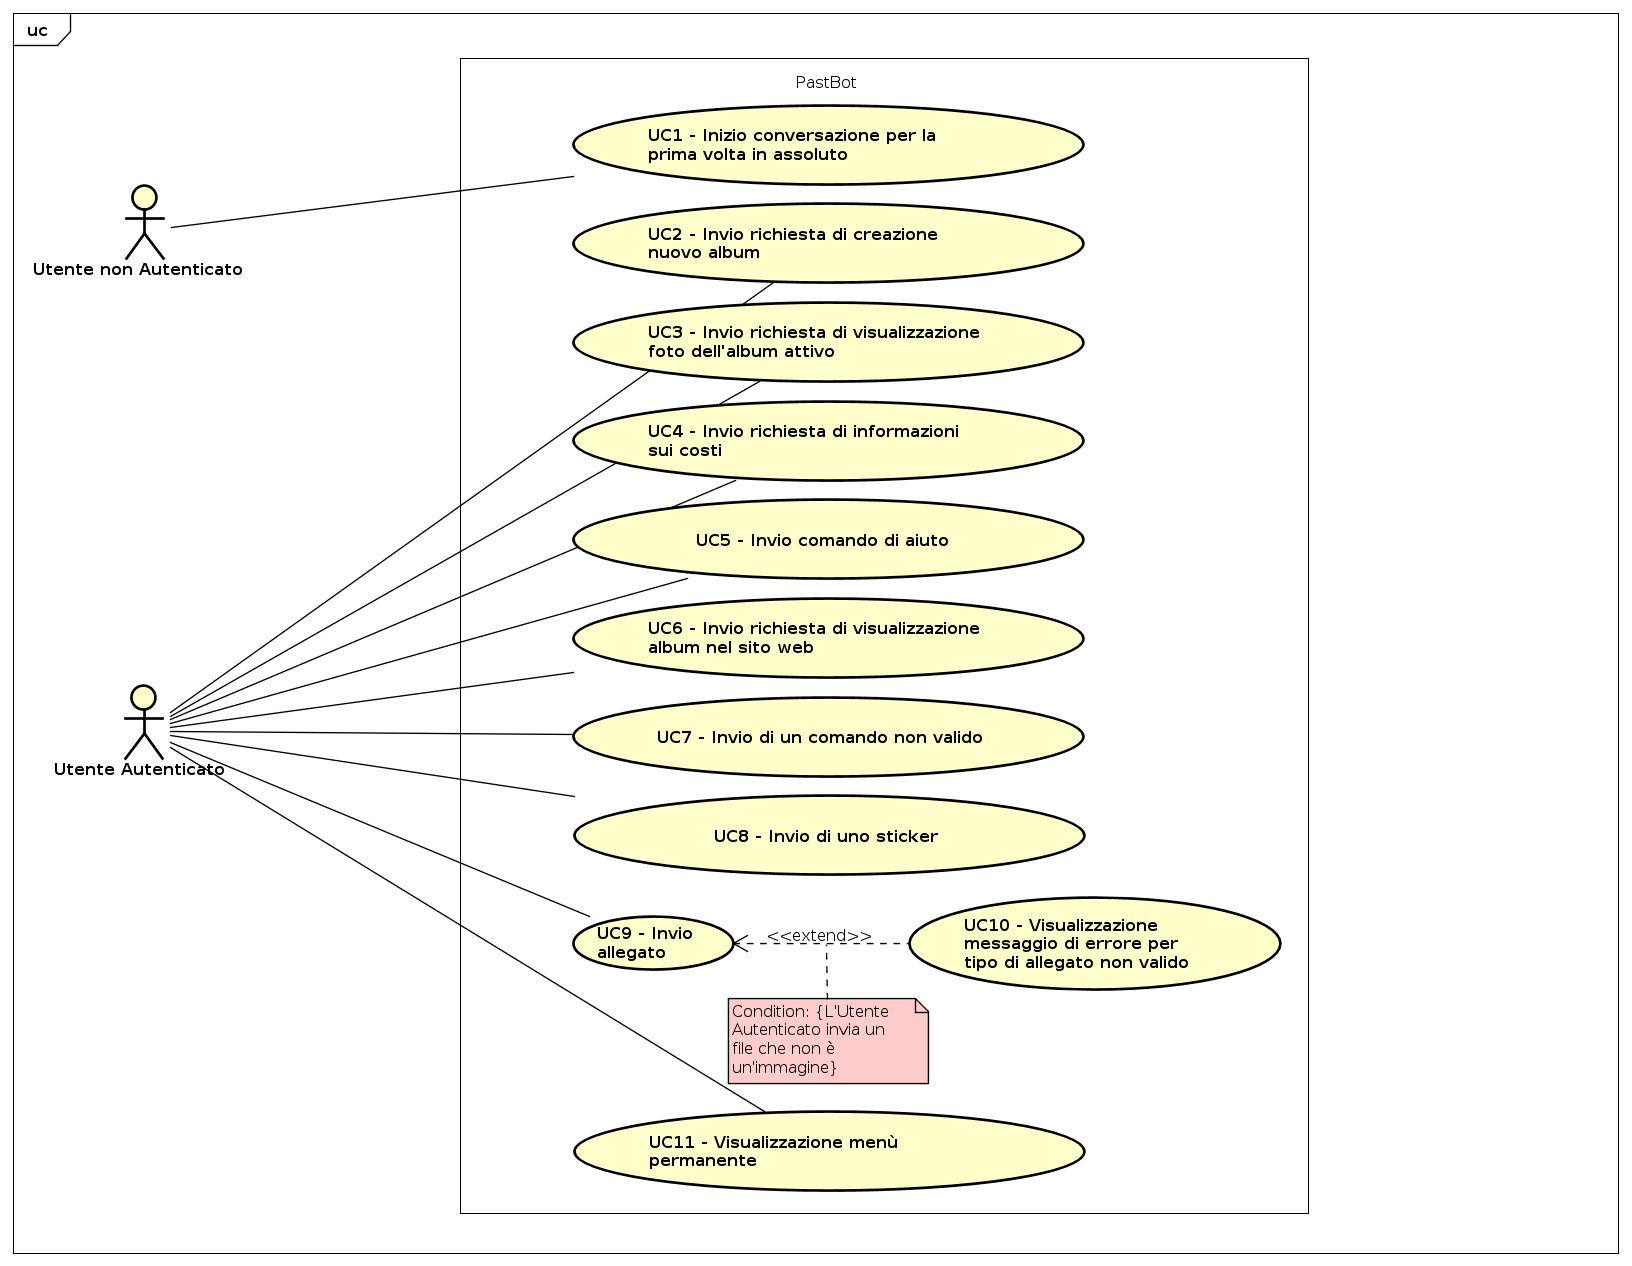
\includegraphics[scale=0.18]{UC0}
  \end{figure}
\end{frame}

\begin{frame}

  \frametitle{Generica API}

  \begin{figure}[H]
    \centering
    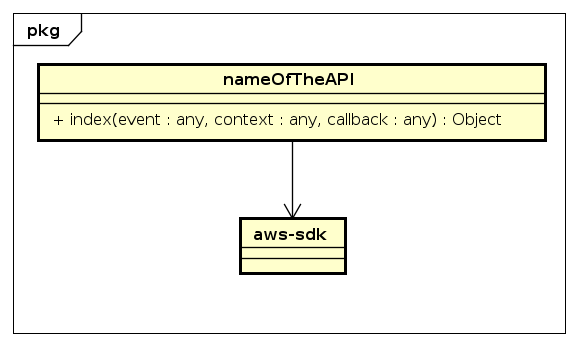
\includegraphics[scale=0.5]{singleAPI}
  \end{figure}
\end{frame}
